
\renewcommand{\EntradaBibtex}{BrazoRobot_Morin2019}
\begin{frame}{\citetitle{\EntradaBibtex} \footnotemark[1] (1)}
%\begin{block}{Brazo Robótico \footnotemark} 
\begin{columns}
	\begin{column}{0.55\textwidth}
		\begin{itemize}
			\item Se retoma un diseño previamente realizado para WebGL. 
			\item Los componentes del robot son movidos mediante motores, y puede ser visto desde difentes perspectivas.		
		\end{itemize}
	\end{column}
	\begin{column}{0.22\textwidth}
		 \begin{center}
		     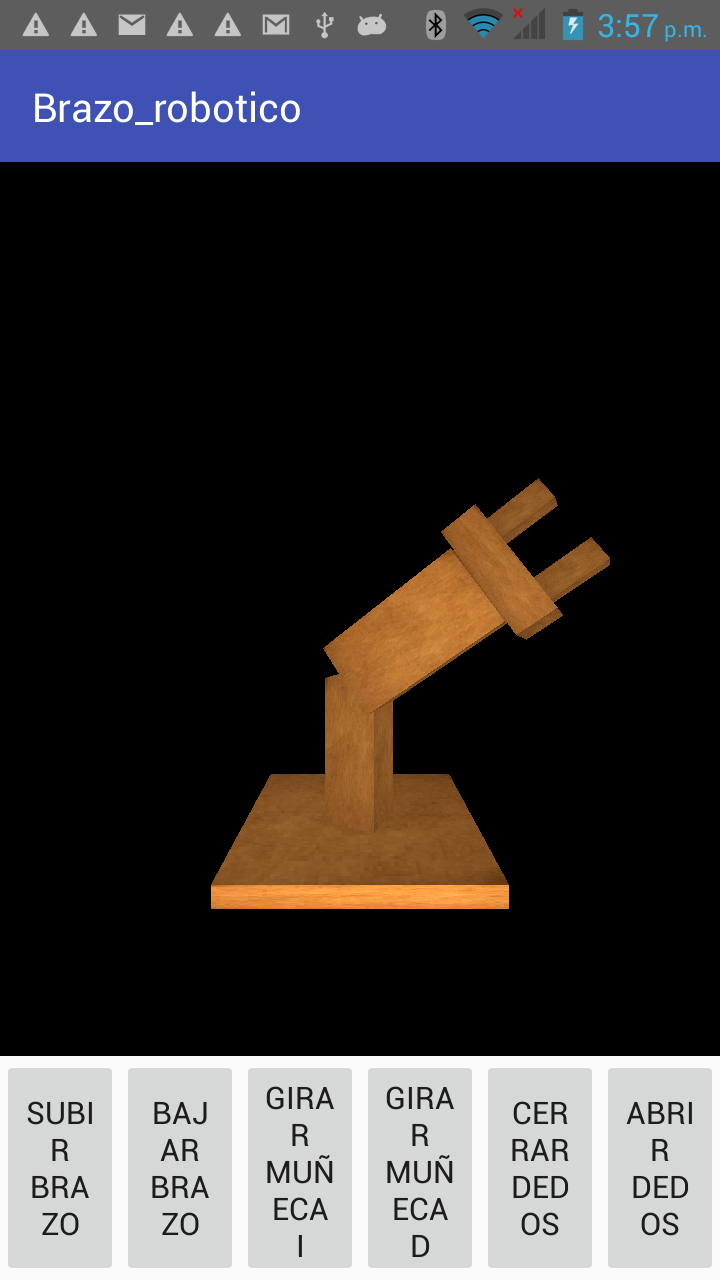
\includegraphics[width=0.98\textwidth]{Figs/brazoRobotico1}
		 \end{center}
	\end{column}
	\begin{column}{0.22\textwidth}  
		\begin{center}
		 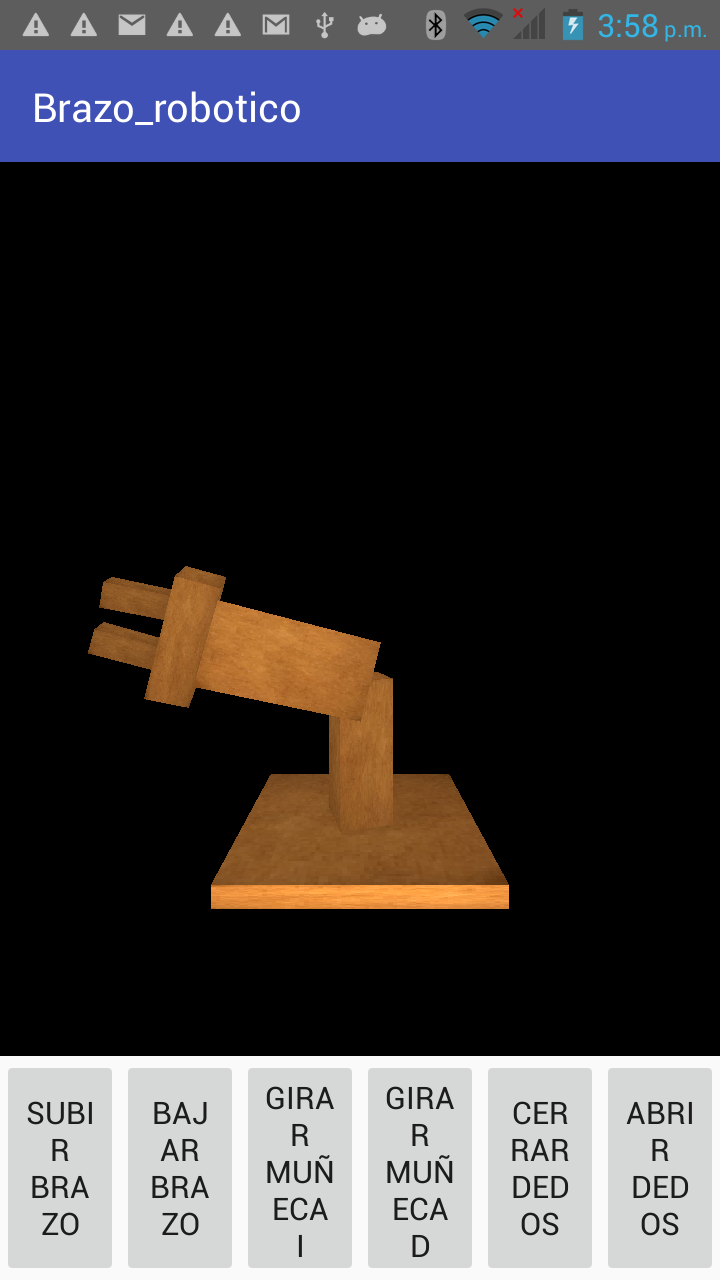
\includegraphics[width=0.98\textwidth]{Figs/brazoRobotico2}
		 \end{center}
	\end{column}
\end{columns}
%\end{block} 
\footnotetext[1]{\fullcite{\EntradaBibtex}}
\end{frame}

\renewcommand{\EntradaBibtex}{BrazoRobot_Uriegas2022}

\begin{frame}{\citetitle{\EntradaBibtex} \footnotemark[1] (1)}
\begin{columns}
\begin{column}{0.25\textwidth}  
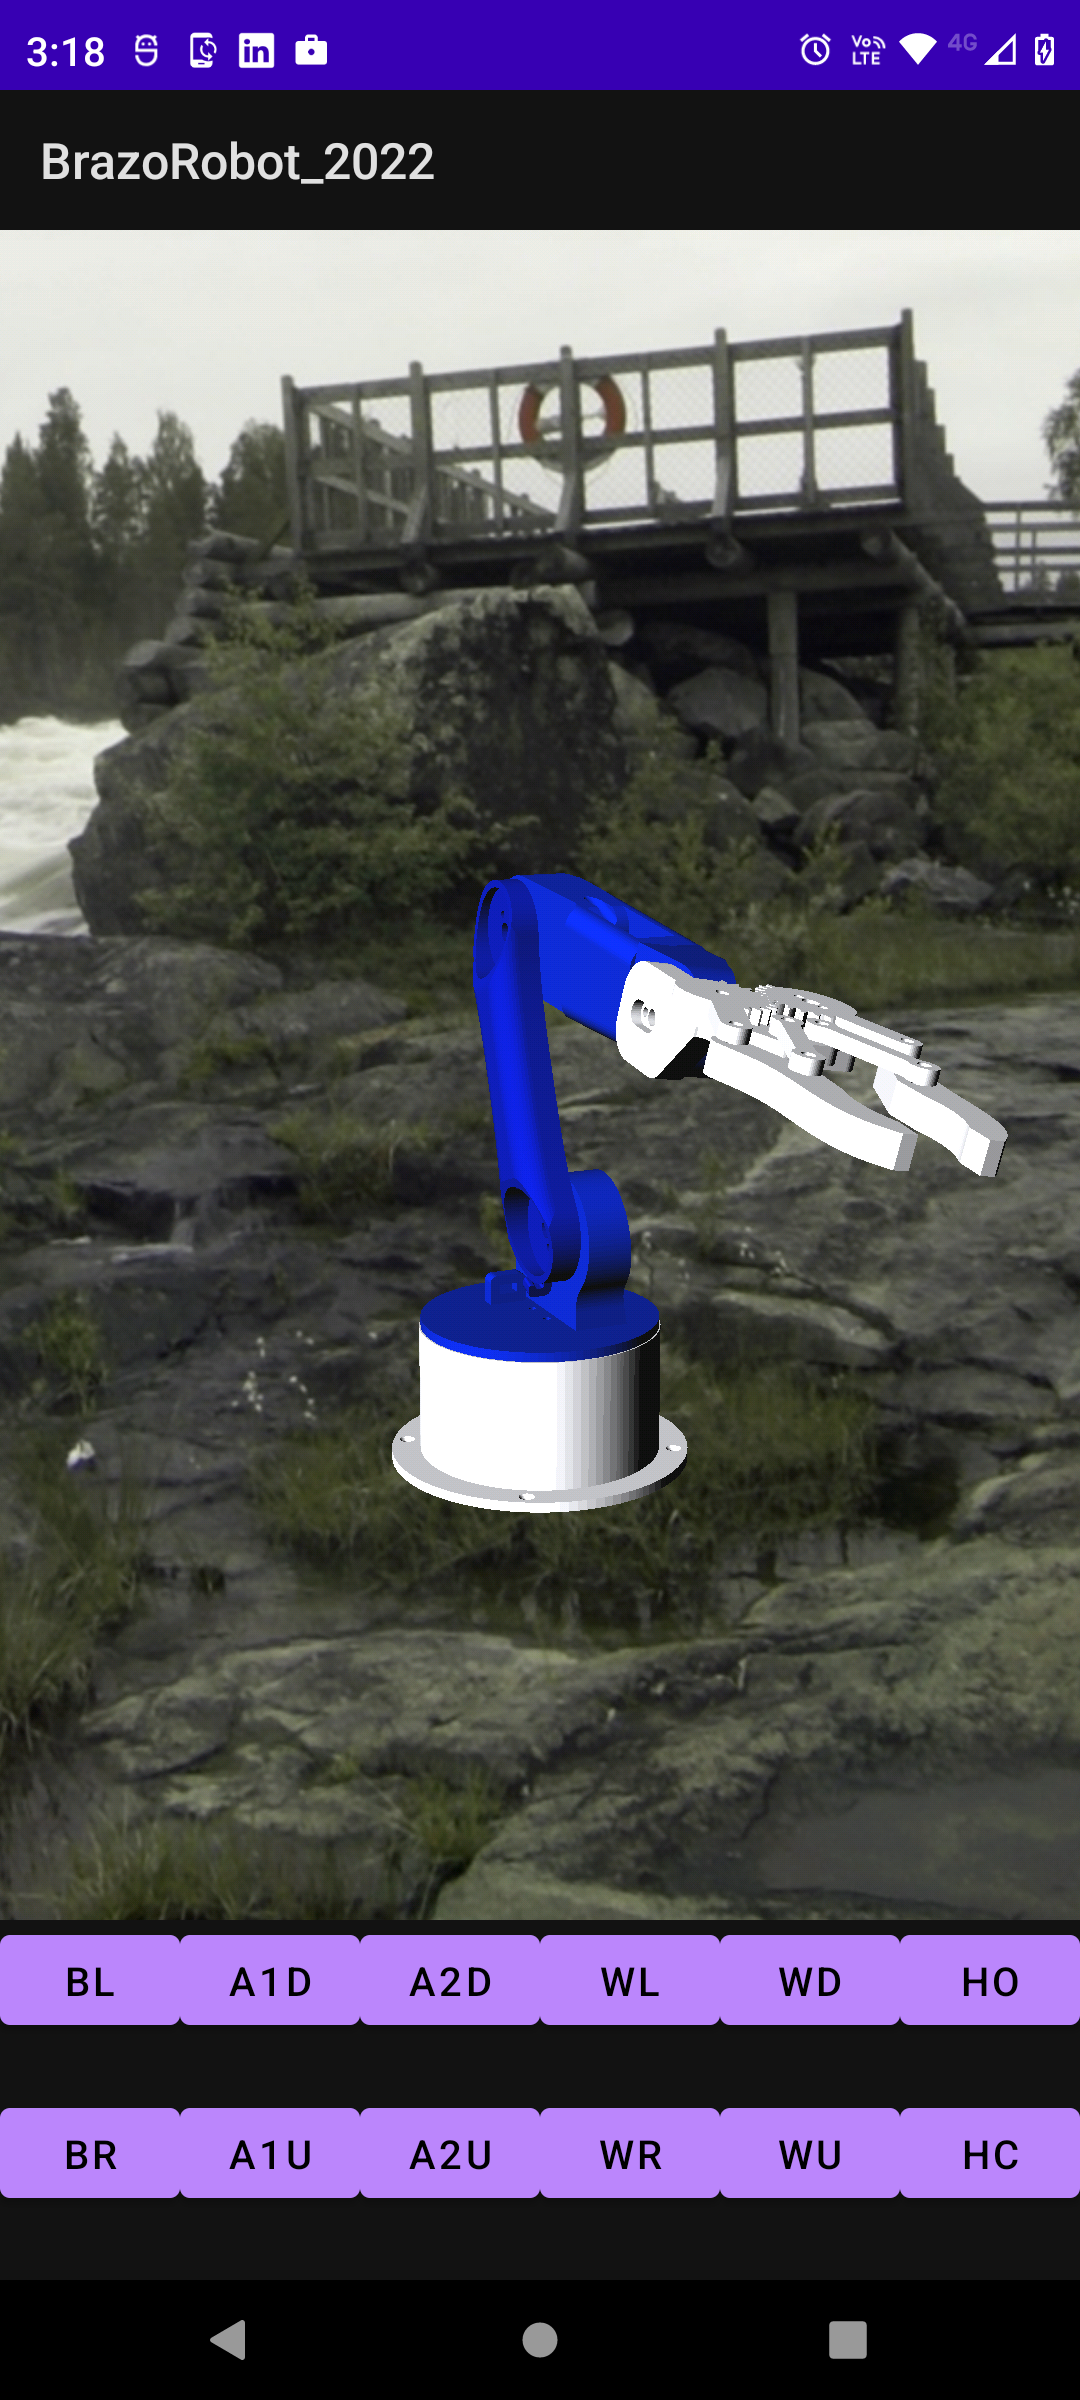
\includegraphics[width=0.82\textwidth]{2019_BrazoRobot3D/figs/BrazoRobot1}
\end{column}
\begin{column}{0.25\textwidth}  
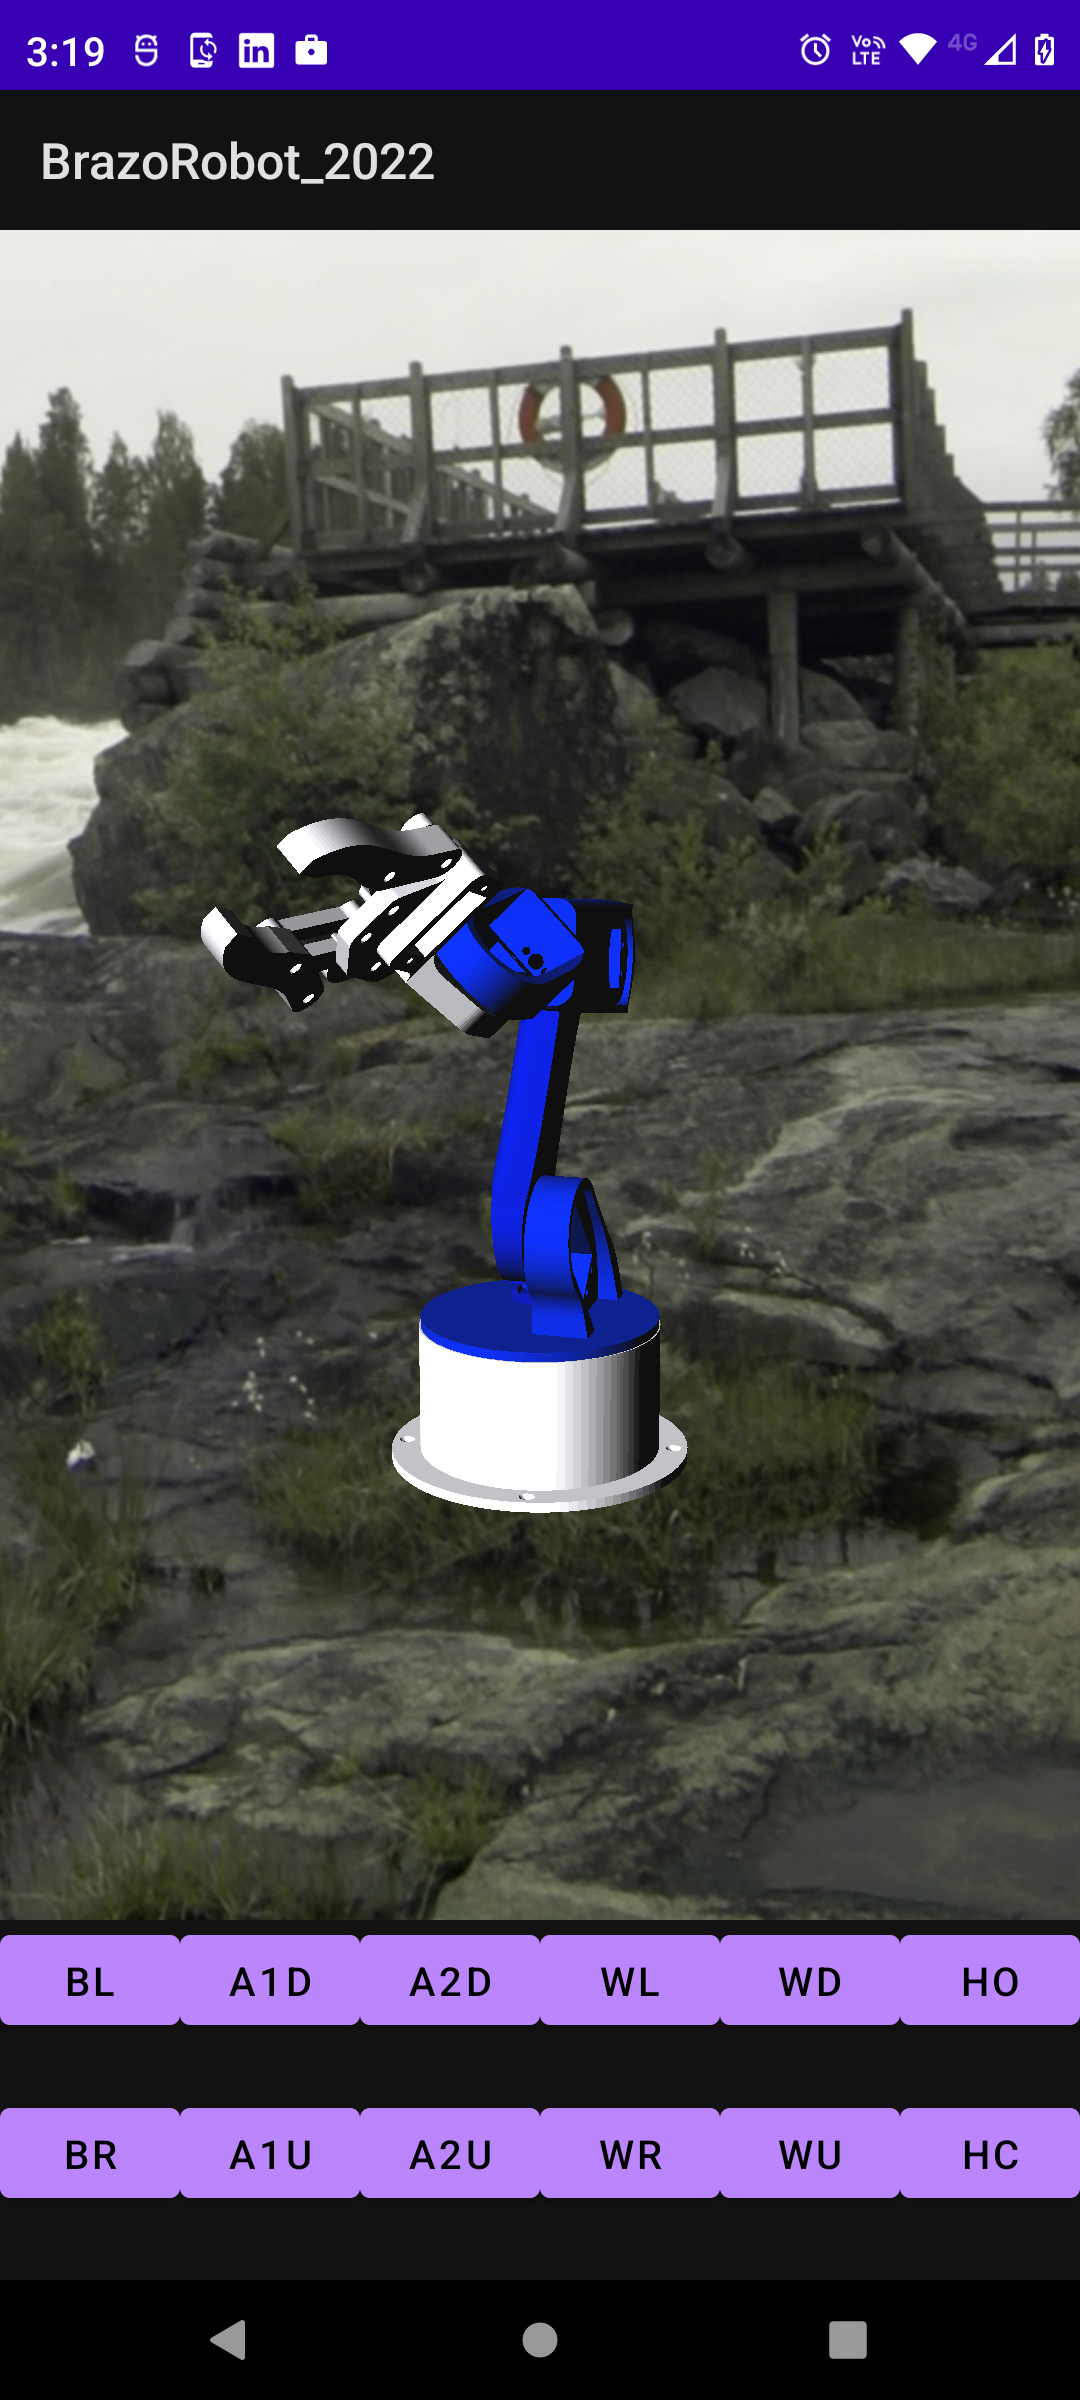
\includegraphics[width=0.82\textwidth]{2019_BrazoRobot3D/figs/BrazoRobot2}
\end{column}
\begin{column}{0.25\textwidth}  
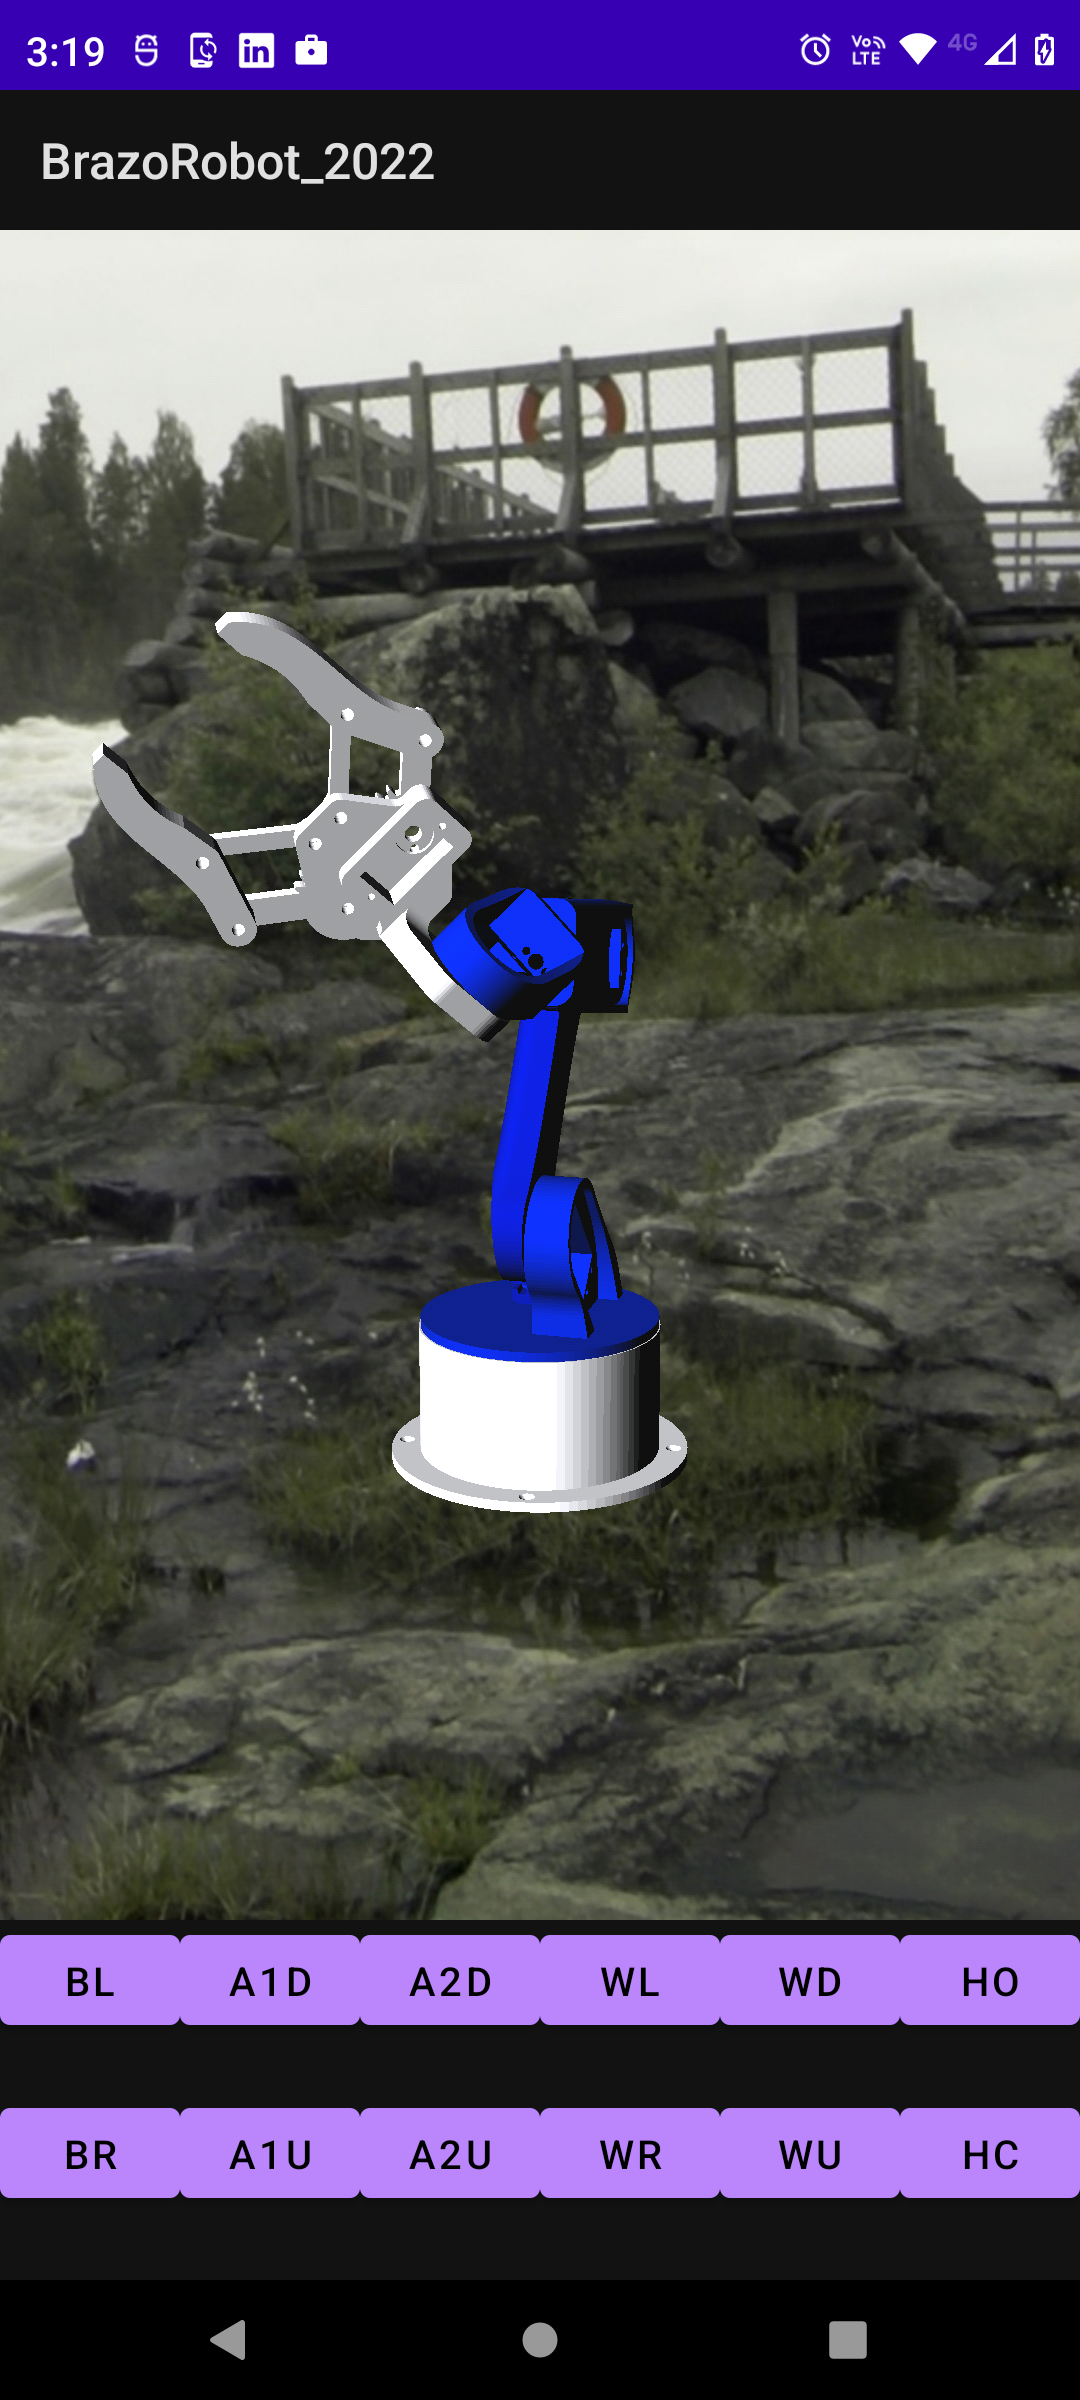
\includegraphics[width=0.82\textwidth]{2019_BrazoRobot3D/figs/BrazoRobot3}
\end{column}
\begin{column}{0.25\textwidth}  
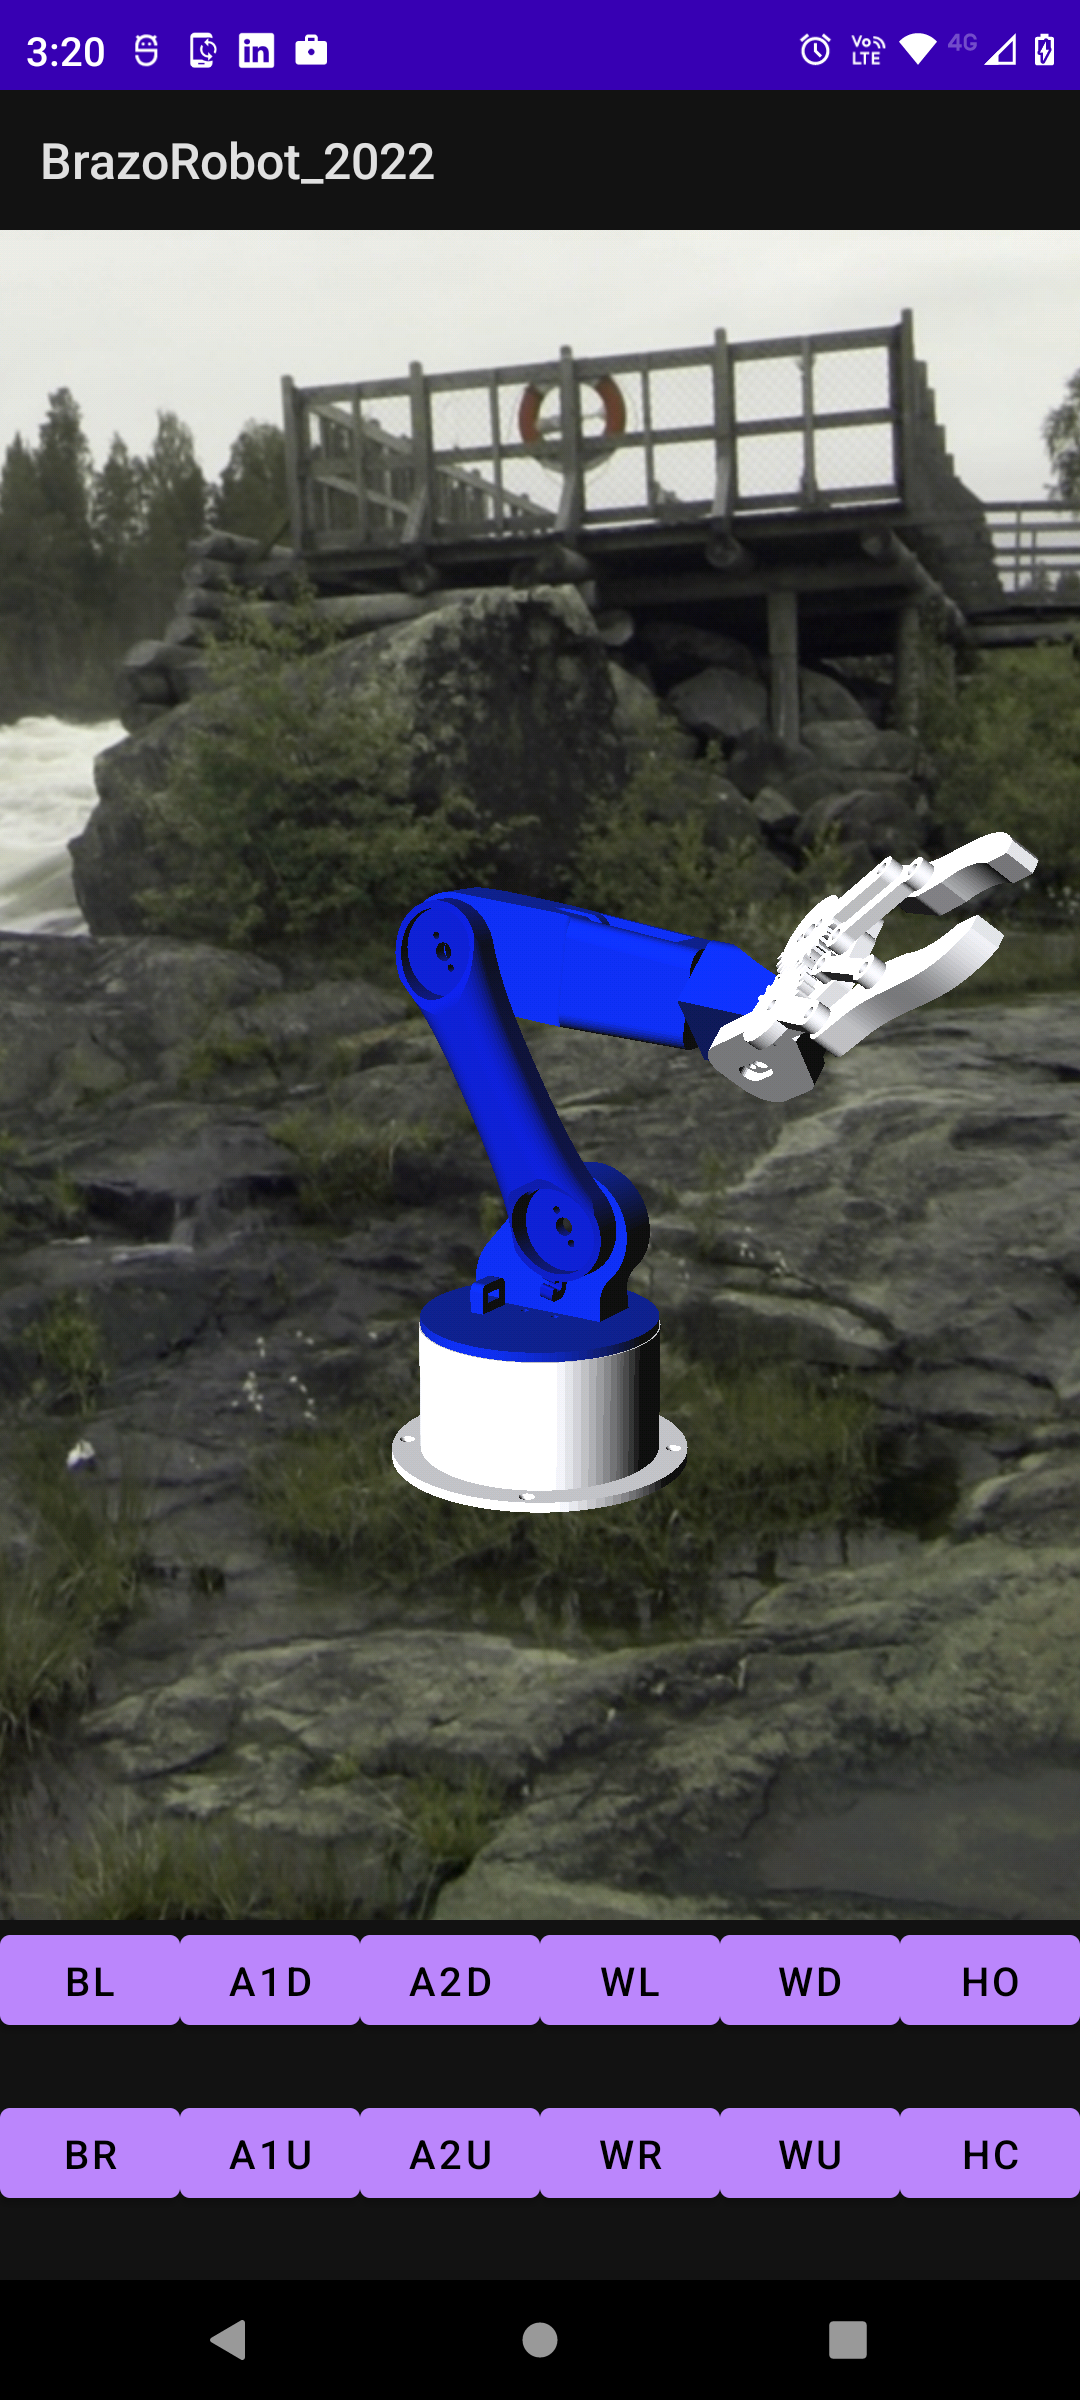
\includegraphics[width=0.82\textwidth]{2019_BrazoRobot3D/figs/BrazoRobot4}
\end{column}

\end{columns}
\footnotetext[1]{\fullcite{\EntradaBibtex}}
\end{frame}

